% Options for packages loaded elsewhere
\PassOptionsToPackage{unicode}{hyperref}
\PassOptionsToPackage{hyphens}{url}
%
\documentclass[
  man,floatsintext]{apa6}
\usepackage{amsmath,amssymb}
\usepackage{iftex}
\ifPDFTeX
  \usepackage[T1]{fontenc}
  \usepackage[utf8]{inputenc}
  \usepackage{textcomp} % provide euro and other symbols
\else % if luatex or xetex
  \usepackage{unicode-math} % this also loads fontspec
  \defaultfontfeatures{Scale=MatchLowercase}
  \defaultfontfeatures[\rmfamily]{Ligatures=TeX,Scale=1}
\fi
\usepackage{lmodern}
\ifPDFTeX\else
  % xetex/luatex font selection
\fi
% Use upquote if available, for straight quotes in verbatim environments
\IfFileExists{upquote.sty}{\usepackage{upquote}}{}
\IfFileExists{microtype.sty}{% use microtype if available
  \usepackage[]{microtype}
  \UseMicrotypeSet[protrusion]{basicmath} % disable protrusion for tt fonts
}{}
\makeatletter
\@ifundefined{KOMAClassName}{% if non-KOMA class
  \IfFileExists{parskip.sty}{%
    \usepackage{parskip}
  }{% else
    \setlength{\parindent}{0pt}
    \setlength{\parskip}{6pt plus 2pt minus 1pt}}
}{% if KOMA class
  \KOMAoptions{parskip=half}}
\makeatother
\usepackage{xcolor}
\usepackage{graphicx}
\makeatletter
\def\maxwidth{\ifdim\Gin@nat@width>\linewidth\linewidth\else\Gin@nat@width\fi}
\def\maxheight{\ifdim\Gin@nat@height>\textheight\textheight\else\Gin@nat@height\fi}
\makeatother
% Scale images if necessary, so that they will not overflow the page
% margins by default, and it is still possible to overwrite the defaults
% using explicit options in \includegraphics[width, height, ...]{}
\setkeys{Gin}{width=\maxwidth,height=\maxheight,keepaspectratio}
% Set default figure placement to htbp
\makeatletter
\def\fps@figure{htbp}
\makeatother
\setlength{\emergencystretch}{3em} % prevent overfull lines
\providecommand{\tightlist}{%
  \setlength{\itemsep}{0pt}\setlength{\parskip}{0pt}}
\setcounter{secnumdepth}{-\maxdimen} % remove section numbering
% Make \paragraph and \subparagraph free-standing
\ifx\paragraph\undefined\else
  \let\oldparagraph\paragraph
  \renewcommand{\paragraph}[1]{\oldparagraph{#1}\mbox{}}
\fi
\ifx\subparagraph\undefined\else
  \let\oldsubparagraph\subparagraph
  \renewcommand{\subparagraph}[1]{\oldsubparagraph{#1}\mbox{}}
\fi
\newlength{\cslhangindent}
\setlength{\cslhangindent}{1.5em}
\newlength{\csllabelwidth}
\setlength{\csllabelwidth}{3em}
\newlength{\cslentryspacingunit} % times entry-spacing
\setlength{\cslentryspacingunit}{\parskip}
\newenvironment{CSLReferences}[2] % #1 hanging-ident, #2 entry spacing
 {% don't indent paragraphs
  \setlength{\parindent}{0pt}
  % turn on hanging indent if param 1 is 1
  \ifodd #1
  \let\oldpar\par
  \def\par{\hangindent=\cslhangindent\oldpar}
  \fi
  % set entry spacing
  \setlength{\parskip}{#2\cslentryspacingunit}
 }%
 {}
\usepackage{calc}
\newcommand{\CSLBlock}[1]{#1\hfill\break}
\newcommand{\CSLLeftMargin}[1]{\parbox[t]{\csllabelwidth}{#1}}
\newcommand{\CSLRightInline}[1]{\parbox[t]{\linewidth - \csllabelwidth}{#1}\break}
\newcommand{\CSLIndent}[1]{\hspace{\cslhangindent}#1}
\ifLuaTeX
\usepackage[bidi=basic]{babel}
\else
\usepackage[bidi=default]{babel}
\fi
\babelprovide[main,import]{english}
% get rid of language-specific shorthands (see #6817):
\let\LanguageShortHands\languageshorthands
\def\languageshorthands#1{}
% Manuscript styling
\usepackage{upgreek}
\captionsetup{font=singlespacing,justification=justified}

% Table formatting
\usepackage{longtable}
\usepackage{lscape}
% \usepackage[counterclockwise]{rotating}   % Landscape page setup for large tables
\usepackage{multirow}		% Table styling
\usepackage{tabularx}		% Control Column width
\usepackage[flushleft]{threeparttable}	% Allows for three part tables with a specified notes section
\usepackage{threeparttablex}            % Lets threeparttable work with longtable

% Create new environments so endfloat can handle them
% \newenvironment{ltable}
%   {\begin{landscape}\centering\begin{threeparttable}}
%   {\end{threeparttable}\end{landscape}}
\newenvironment{lltable}{\begin{landscape}\centering\begin{ThreePartTable}}{\end{ThreePartTable}\end{landscape}}

% Enables adjusting longtable caption width to table width
% Solution found at http://golatex.de/longtable-mit-caption-so-breit-wie-die-tabelle-t15767.html
\makeatletter
\newcommand\LastLTentrywidth{1em}
\newlength\longtablewidth
\setlength{\longtablewidth}{1in}
\newcommand{\getlongtablewidth}{\begingroup \ifcsname LT@\roman{LT@tables}\endcsname \global\longtablewidth=0pt \renewcommand{\LT@entry}[2]{\global\advance\longtablewidth by ##2\relax\gdef\LastLTentrywidth{##2}}\@nameuse{LT@\roman{LT@tables}} \fi \endgroup}

% \setlength{\parindent}{0.5in}
% \setlength{\parskip}{0pt plus 0pt minus 0pt}

% Overwrite redefinition of paragraph and subparagraph by the default LaTeX template
% See https://github.com/crsh/papaja/issues/292
\makeatletter
\renewcommand{\paragraph}{\@startsection{paragraph}{4}{\parindent}%
  {0\baselineskip \@plus 0.2ex \@minus 0.2ex}%
  {-1em}%
  {\normalfont\normalsize\bfseries\itshape\typesectitle}}

\renewcommand{\subparagraph}[1]{\@startsection{subparagraph}{5}{1em}%
  {0\baselineskip \@plus 0.2ex \@minus 0.2ex}%
  {-\z@\relax}%
  {\normalfont\normalsize\itshape\hspace{\parindent}{#1}\textit{\addperi}}{\relax}}
\makeatother

% \usepackage{etoolbox}
\makeatletter
\patchcmd{\HyOrg@maketitle}
  {\section{\normalfont\normalsize\abstractname}}
  {\section*{\normalfont\normalsize\abstractname}}
  {}{\typeout{Failed to patch abstract.}}
\patchcmd{\HyOrg@maketitle}
  {\section{\protect\normalfont{\@title}}}
  {\section*{\protect\normalfont{\@title}}}
  {}{\typeout{Failed to patch title.}}
\makeatother

\usepackage{xpatch}
\makeatletter
\xapptocmd\appendix
  {\xapptocmd\section
    {\addcontentsline{toc}{section}{\appendixname\ifoneappendix\else~\theappendix\fi\\: #1}}
    {}{\InnerPatchFailed}%
  }
{}{\PatchFailed}
\keywords{language development; blindness; vocabulary\newline\indent Word count: X}
\usepackage{csquotes}
\ifLuaTeX
  \usepackage{selnolig}  % disable illegal ligatures
\fi
\IfFileExists{bookmark.sty}{\usepackage{bookmark}}{\usepackage{hyperref}}
\IfFileExists{xurl.sty}{\usepackage{xurl}}{} % add URL line breaks if available
\urlstyle{same}
\hypersetup{
  pdftitle={The Role of Vision in the Acquisition of Words: Vocabulary Development in Blind Toddlers},
  pdfauthor={Erin Campbell1, Robyn Casillas2, \& Elika Bergelson1},
  pdflang={en-EN},
  pdfkeywords={language development; blindness; vocabulary},
  hidelinks,
  pdfcreator={LaTeX via pandoc}}

\title{The Role of Vision in the Acquisition of Words: Vocabulary Development in Blind Toddlers}
\author{Erin Campbell\textsuperscript{1}, Robyn Casillas\textsuperscript{2}, \& Elika Bergelson\textsuperscript{1}}
\date{}


\shorttitle{Vocabulary Production of Blind Toddlers}

\authornote{

Correspondence concerning this article should be addressed to Erin Campbell, 417 Chapel Drive, Durham, NC, 27708. E-mail: \href{mailto:erin.e.campbell@duke.edu}{\nolinkurl{erin.e.campbell@duke.edu}}

}

\affiliation{\vspace{0.5cm}\textsuperscript{1} Duke University\\\textsuperscript{2} Independent Researcher}

\note{

\textbf{Conflicts of Interest}: The authors have no conflicts of interest to report.
\textbf{Funding}: This work was supported by the National Science Foundation CAREER grant (BCS-1844710) to EB and Graduate Research Fellowship (2019274952) to EC.
\textbf{Data Availability}: The data and code used to generate this paper on \href{https://osf.io/uw6zm/?view_only=fdee466143f64d678d7f9d87b23ec566}{OSF}, which will be made publically accessible following acceptance of the manuscript.
\textbf{Ethics Approval}: This study received approval from Duke University Institutional Review Board.

}

\begin{document}
\maketitle

\hypertarget{research-highlights}{%
\section{Research Highlights}\label{research-highlights}}

\begin{itemize}
\tightlist
\item
  Infants and toddlers born blind (with no other diagnoses) show a 7.5 month productive vocabulary delay on average, with wide variability.
\item
  Across the studied age range (7-57mo.), vocabulary delays widened with age.
\item
  Blind and sighted children's early vocabularies contain similar distributions of word lengths, parts of speech, semantic categories, and perceptual modalities.
\item
  Blind children (but not sighted children) were more likely to say visual words which could also be experienced through other senses.
\end{itemize}

\hypertarget{abstract}{%
\section{Abstract}\label{abstract}}

What is vision's role in driving early word production? To answer this, we assessed parent-report vocabulary questionnaires administered to congenitally blind children (N = 40, Mean age = 24mo.(R: 7-57mo.)) and compared the size and contents of their productive vocabulary to those of a large normative sample of sighted children (N=6574). We found that on average, blind children showed a roughly half-year vocabulary delay relative to sighted children, amid considerable variability. However, the content of blind and sighted children's vocabulary was statistically indistinguishable in word length, part of speech, semantic category, concreteness, interactiveness, and perceptual modality. At a finer-grained level, we also found that words' perceptual properties intersect with children's perceptual abilities. Our findings suggest that while an absence of visual input may initially make vocabulary development more difficult, the content of the early productive vocabulary is largely resilient to differences in perceptual access.

\hypertarget{introduction}{%
\section{Introduction}\label{introduction}}

Descriptions of early word learning often invoke visual scenes: a messy living room, a rabbit jumping across a trail. At some level, word learners are thought to take the linguistic input, deduce referents in a visual sea of possibilities, and connect this input to intended meaning. How do young learners do this? Some propose they look for visually salient objects (Yu \& Smith, 2012); others suggest central roles for following speakers' gaze or intent (Brooks \& Meltzoff, 2008; Tomasello, 2003). These strategies could help constrain referent possibilities given a novel word and ambiguous visual input, but such approaches do not work for all words, let alone all learners.

If visual input is integral to word learning, then its absence should lead to pronounced differences in language abilities. However, blind adults perform comparably to sighted adults on many language tasks, and on some tasks, demonstrate faster language processing than sighted adults (Bottini, Morucci, D'Urso, Collignon, \& Crepaldi, 2022; Loiotile, Lane, Omaki, \& Bedny, 2020; Röder, Demuth, Streb, \& Rösler, 2003). But are these equivalencies or advantages present in the earliest stages of language development, or do they emerge over time? One way to tackle this question is to study vocabulary development in congenitally blind children. We ask: does a radically different experience of perceiving the world lead to differences in how we begin to learn words?

\hypertarget{potential-challenges-for-the-blind-learner.}{%
\subsection{Potential Challenges for the Blind Learner.}\label{potential-challenges-for-the-blind-learner.}}

Though blind adults are skilled language users, the nature of their early lexicon (in terms of vocabulary size and composition) remains unclear. Before returning to this, we discuss several social and motor supports of early language development for sighted children that are absent or delayed in blind children.

Social interaction provides one potential support for children's early word learning. Parents often talk about what they or their child are looking at (Tomasello, 2003; Yurovsky, Smith, \& Yu, 2013), and such naming events have been linked with better word learning (Pereira, Smith, \& Yu, 2014), (though n.b., such labeling events are still relatively infrequent, Clerkin, Hart, Rehg, Yu, \& Smith, 2017; Clerkin \& Smith, 2022). In turn, following speakers' gaze may help children deduce communicative intent (Brooks \& Meltzoff, 2008; Carpenter, Nagell, Tomasello, Butterworth, \& Moore, 1998; Meltzoff \& Brooks, 2009). In sighted infants, gaze-following is linked with later vocabulary size (Brooks \& Meltzoff, 2008). However, in blind infants, gaze-following is not an accessible cue to deduce word meaning, and neither can parents reliably use blind children's gaze to provide language input tailored to the locus of their attention.

The abilities to reach for, grasp, and manipulate objects of interest have been proposed as another set of supports for word learning. For instance, words with easily manipulable referents are more frequent in children's early productive vocabulary than non-manipulable ones (e.g.~cup vs.~table, Nelson, 1973), and ratings of the extent to which children can physically interact with word referents predict words' age of acquisition (Muraki, Siddiqui, \& Pexman, 2022). Additionally, like gaze, children's object manipulation may highlight children's attentional focus for parents, eliciting more object naming (Luo \& Tamis-LeMonda, 2016; Tamis-LeMonda, Kuchirko, \& Tafuro, 2013; K. L. West \& Iverson, 2017; M. J. West \& Rheingold, 1978). When a parent provides a label for an object a child is manipulating, that referent is likely to be highly perceptually salient, as held objects dominate infants' visual field (Yu \& Smith, 2012). Taken together, these lines of work suggest infants' object manipulation could (perhaps in conjunction with other word or object features) support word learning by providing the infant with perceptual information about the object, as well as cuing parents in to what their child is attending.

However, in blind children, grasping and reaching are delayed (Fraiberg \& Fraiberg, 1977; Norris, 1957; Perez-Pereira \& Conti-Ramsden, 1999): While sighted children reach towards a seen object at around 2.5--5.5 weeks of age (Adolph \& Robinson, 2015; Berthier \& Keen, 2006; Clifton, Muir, Ashmead, \& Clarkson, 1993), with prereaching behaviors observable even earlier (Smitsman \& Corbetta, 2010), a parallel ability, reaching towards an object making noise, does not emerge in blind infants until around 8-12 months, similar to sighted children's timeline for hand-ear coordination (Bigelow, 1986; Elisa et al., 2002; Fraiberg \& Fraiberg, 1977; Tröster \& Brambring, 1993).

Likewise, pointing is linked with children's language ability (Colonnesi, Stams, Koster, \& Noom, 2010; C. Moore, Dailey, Garrison, Amatuni, \& Bergelson, 2019), perhaps because it too directs a conversation partner's attention. Sighted infants shift their gaze to the direction of a point reliably by around 10--12 months of age (Carpenter et al., 1998) and begin pointing themselves at around the same age (C. Moore et al., 2019). Pointing is argued to support word learning by serving as a naming ``request'' (Lucca \& Wilbourn, 2019); by 18 months, labels given after infants point are better learned (Lucca \& Wilbourn, 2018). By contrast, in naturalistic settings, an analysis of 5 blind children aged 14--24-months found that they engaged less frequently in pointing than sighted peers, opting instead for gesturing with an open palm towards proximal objects (Iverson, Tencer, Lany, \& Goldin-Meadow, 2000). However, it is worth noting that the relationship between this behavior and its impact on word learning has not yet been thoroughly tested due to the limited available research in this area.

Reaching, gaze-following, and pointing also serve as useful cues for establishing joint attention, wherein two individuals are simultaneously focused on each other and an object or event. Joint attention may provide referentially transparent language input, which can facilitate word learning (Tomasello \& Farrar, 1986). For blind children however, joint attention is often delayed relative to sighted peers (Bigelow, 2003; Perez-Pereira \& Conti-Ramsden, 1999), (even more so for those with no residual vision, Dale, Tadić, \& Sonksen, 2014). If reaches, gazes, and points help cue parents to their infants' interest, and if these cues are delayed or unavailable for parents of blind infants, then blind infants may not receive language input that is as temporally-aligned with their attention as a sighted child would (cf. Trueswell et al., 2016). This may reduce the number of labeling instances with high referential clarity available to blind children, thus limiting word learning through this particular mechanism.

\hypertarget{vocabulary-development-in-blind-children.}{%
\subsection{Vocabulary Development in Blind Children.}\label{vocabulary-development-in-blind-children.}}

The potential challenges for blind learners enumerated above are intended to showcase the various avenues by which vision could potentially influence early word learning. While none of these skills (grasping, pointing, reaching, gaze) are necessarily critical for the learning of any given word, each appears to offer support in certain word learning circumstances. If the highlighted skills are indeed important supports to word learning, we might expect concomitant language delays or deficits in blind children. However, prior work on productive vocabulary development in this population is inconclusive. Some research finds that blind infants learn words on roughly the same timeline as sighted infants (Landau \& Gleitman, 1985; Wilson \& Halverson, 1947); others find delays in first-word production (Brambring, 2007; Fraiberg \& Fraiberg, 1977; Iverson et al., 2000; V. Moore \& McConachie, 1994; Mulford, 1988). The existence and extent of vocabulary delays may of course be influenced by a host of other factors, such as severity of the vision diagnosis, etiology, comorbid diagnoses, etc. (Greenaway \& Dale, 2017). Understanding which blind children may be at particular risk for language deficits or delays remains an important clinical goal.

\hypertarget{vocabulary-composition}{%
\subsubsection{Vocabulary Composition}\label{vocabulary-composition}}

The composition of blind children's first words has been reported as largely similar to that of sighted children. Like English-learning sighted children, English-learning blind children's first words include a large proportion of nouns (Andersen, Dunlea, \& Kekelis, 1984; Bigelow, 1986; Dunlea, 1989; Landau \& Gleitman, 1985). Some studies have found that blind children may have a weaker noun bias (Mcconachie \& Moore, 1994; Mulford, 1988; Norgate, 1997), which may be due to fewer ``point-and-look'' learning episodes relative to sighted children (Norgate, 1997); others report fewer words for distal objects (e.g.~outdoor objects and animals, Bigelow, 1987). These differences in vocabulary composition are small in magnitude and inconsistent across the literature. More strikingly, despite lacking visual access, blind children preschool age and up have been reported to use visual terms like ``red'' (DeMott, 1972; Harley, 1963; Landau \& Gleitman, 1985). These findings underscore the potential complexity of vocabulary composition in blind children and highlight the need for a multidimensional approach to explore the intricacies of their early word learning experiences.

While existing research on vocabulary development in blind children provides a valuable foundation, each of the studies cited above is based on a limited sample size, typically N\textless10. This stems from the challenges of sampling young blind children without additional cognitive deficits; congenital blindness often occurs as part of syndromes with wide-ranging symptoms (e.g., Garcia-Filion \& Borchert, 2013). Expanding this work is an important goal, both for improving early intervention services for blind children, as well as better understanding how visual perception contributes to word learning more broadly. In what follows, we explore the role of vision in word learning using a standardized vocabulary measure administered to 40 blind children. We ask whether blind children have productive vocabulary differences relative to their sighted peers, both in quantity (i.e.~how many words they produce), and composition (i.e.~which words they produce).

\hypertarget{methods}{%
\section{Methods}\label{methods}}

Approximately 1/10,000 children is born with severe to profound visual impairment (Gilbert \& Awan, 2003); congenital blindness is a low incidence condition. Our sample includes 40 young, congenitally blind children (7--57 months, M: 24.01 (12.46) months). To focus specifically on the role of vision in language development, children met inclusion criteria if they (1) were exposed to \textgreater75\% English at home, (2) had \emph{no more than minimal light perception} in both eyes, (3) had no co-occurring cognitive or developmental diagnoses, and (4) had no history of frequent ear infections or hearing loss; see Table \ref{tab:diagnosis-table} for vision diagnosis specifics. Data from 3 participants were collected but excluded due to bilingualism (N=2), hearing loss (N=2), and/or co-occurring cognitive or developmental diagnoses (N=1). Participants were recruited in the United States and Canada via pediatric ophthalmology clinics, early intervention and preschool programs for blind children, social media, and word of mouth. Many participants contributed data at multiple timepoints, for a total of N=70 total datapoints (1--5 per child, M: 1.75); to avoid overrepresenting participants, we use only data from the oldest timepoint for analyses, except in the longitudinal analysis, noted below. Data from 11 participants were originally described in Herrera (2015). Participant demographics are available in Table \ref{tab:demographics-table}.

\begin{table}[H]

\caption{\label{tab:diagnosis-table}Severity of visual impairment and vision diagnoses for each blind child in the sample.}
\centering
\begin{tabular}[t]{l|r|r|r|l}
\hline
Diagnosis & N severe & N profound & N severity unspecified & Etiology\\
\hline
Optic Nerve Hypoplasia & 8 & 3 & 0 & Central\\
\hline
Not specified & 2 & 2 & 3 & \\
\hline
Leber's Congenital Amaurosis & 3 & 1 & 0 & Peripheral\\
\hline
Cataracts & 3 & 0 & 0 & Peripheral\\
\hline
Microphthalmia & 3 & 0 & 0 & Peripheral\\
\hline
Anopthalmia & 0 & 2 & 0 & Peripheral\\
\hline
Multiple & 2 & 0 & 0 & \\
\hline
Ocular albinism & 1 & 1 & 0 & Peripheral\\
\hline
Retinal Detachments & 1 & 1 & 0 & Peripheral\\
\hline
CVI & 1 & 0 & 0 & Central\\
\hline
Fused Eyelids & 1 & 0 & 0 & Peripheral\\
\hline
Optic Pathway Glioma & 1 & 0 & 0 & Central\\
\hline
Retinopathy of Prematurity & 0 & 1 & 0 & Peripheral\\
\hline
\end{tabular}
\end{table}

\begin{table}[H]

\begin{threeparttable}
\caption{\label{tab:demographics-table}Demographic characteristics of the 40 blind participants in the study.}
\centering
\begin{tabular}[t]{l|>{\raggedright\arraybackslash}p{4in}}
\hline
Variable & Range and Mean, or Ns\\
\hline
Age (months) & 7-57 months (mean (SD): 24.01 (12.46))\\
\hline
Receptive Vocabulary* (CDI) & 0-391 words (mean (SD): 59.94 (80.92))\\
\hline
Productive Vocabulary (CDI) & 0-680 words (mean (SD): 141.8 (223.91))\\
\hline
Gender & Female (15); Male (25)\\
\hline
Maternal Education & High School (2); Associates Degree or Some College (11); Bachelors degree (18); Graduate degree (8), Missing (1)\\
\hline
Child Race & American Indian or Alaska Native (1); Black or African American (5); Southeast Asian or Indian (1); White (20); Multiracial or Other (2); Missing data (11)\\
\hline
Child Ethnicity & Hispanic or Latino (4); Not Hispanic or Latino (23); Missing data (13)\\
\hline
\end{tabular}
\begin{tablenotes}
\small
\item [*] Receptive vocabulary scores only measured on Words and Gestures version of CDI; all Words and Sentences administrations excluded from these values.
\end{tablenotes}
\end{threeparttable}
\end{table}

Parents of each child in our sample completed the MacArthur-Bates Communicative Development Inventory (CDI). The CDI is a parent-report instrument predominantly used to assess children's productive/receptive vocabulary alongside a few items regarding other aspects of early language; we focus on the vocabulary data here. On the Words and Gestures version of the form (WG; normed for 8--18-month-olds), parents indicate whether their child understands and/or produces each of the 398 vocabulary items. On the Words and Sentences version (WS; normed for 16--30-month-olds\footnote{For 16--18-month-olds, where it was ambiguous which CDI version to take, children were given WG if it was their first administration, or if previous administrations showed that they were not yet producing many words. If children were producing \textgreater50 words on a previous administration, they were given WS.}), parents indicate whether their child produces each of the 680 vocabulary items. Parents of blind children in our study were first administered the CDI when initially recruited (which varied considerably in age) and then at 6 month intervals (at 12, 18, 24,\ldots., 48 months); longitudinal data collection is ongoing.

Normative data for the CDI is available from English and many other languages on WordBank (e.g., Frank, Braginsky, Yurovsky, \& Marchman, 2017), an open database of CDI data. While the CDI has not been validated for blind children, it has been used successfully in other special populations, such as Deaf/Hard-of-Hearing children (Thal, Desjardin, \& Eisenberg, 2007), late talkers (Heilmann, Weismer, Evans, \& Hollar, 2005), and children with Down syndrome (Miller, Sedey, \& Miolo, 1995). Critically, in many of these populations, the CDI production measure has been validated for ``off-label'' usage above the chronological age for which the CDI has been normed for typically-developing children (Heilmann et al., 2005; Miller et al., 1995; Thal et al., 2007).

\hypertarget{results}{%
\section{Results}\label{results}}

\hypertarget{analysis-plan}{%
\subsection{Analysis Plan}\label{analysis-plan}}

Our results are organized around answering the two questions set out above: do blind and sighted children differ in how many words they say at a given age, and do they differ in the composition of those vocabularies. To address the first question, we compared blind children's vocabulary on the CDI relative to norms derived from sighted children of the same age. We then considered a variety of child-level characteristics to get a better understanding of what may contribute to the overall delay we observe, as well as an analysis of delay size with age. For these analyses we used logistic regression curves, Wilcoxon Tests, and linear regression, as relevant. To address the second question, we matched for vocabulary size and compared blind and sighted children's vocabulary composition across a range of factors: word length, part of speech, semantic category, concreteness, interactiveness, and perceptual modality (details below). For these analyses we used Bonferroni-corrected Wilcoxon Tests and logistic regressions. Previewing the results to this question, we found evidence of vocabulary delays among blind children but very consistent vocabulary composition across our blind and sighted groups. We describe the findings in full detail below, and provide the data and code used to generate this paper on \href{https://osf.io/uw6zm/?view_only=fdee466143f64d678d7f9d87b23ec566}{OSF}. These analyses were not preregistered.

\hypertarget{do-blind-children-and-sighted-children-have-similar-vocabulary-sizes}{%
\subsection{Do blind children and sighted children have similar vocabulary sizes?}\label{do-blind-children-and-sighted-children-have-similar-vocabulary-sizes}}

To analyze whether blind children produce a similar \emph{quantity} of words to their sighted peers, we used a large set of vocabulary production data from Wordbank. The normative dataset contains data from 6574 children (8-30 mo., who range in vocabulary from producing none of the words on the instrument to producing all words on the instrument) learning American English (downloaded 2022-11-05 from \href{http://wordbank.stanford.edu/data?name=vocab_norms}{Wordbank}). As noted above, the two CDI forms differ in how many vocabulary items they contain. To take this into account, we established the difference (in months) between the child's chronological age and their predicted age based on their productive vocabulary, derived from the WordBank norms (Frank et al., 2017), rather than using the raw number of words checked off on the instrument.

Following the procedure in Campbell \& Bergelson (2022), to compute a child's predicted age from their vocabulary score, we used the Wordbank's 50th percentile for productive vocabulary for sighted infants (Frank et al., 2017) to create two binary logistic growth curves (for the WG and WS versions of the CDI). For each child, we took their productive vocabulary score, as reported on the CDI. We then divided the number of words produced by the number of possible words on the instrument (WG or WS), to give us the proportion of words produced. We used this proportion in an inverse prediction from the binary logistic regression curves to generate a predicted age. That is, for each possible CDI score, the growth curve provided the age that the score would be achieved for the 50th percentile trajectory. Finally, we subtracted the predicted age from each child's chronological age to calculate their vocabulary delay or advantage. For instance, a 30-month-old blind child producing 300 words has the vocabulary size of a 25-month-old sighted child at the 50th percentile, and would thus have a vocabulary difference of 5 months relative to the Wordbank data; see Figure \ref{fig:growth-curve-illustration} for a visual representation of this procedure. However, for children producing 0 words (N=9), this approach is not appropriate due to the long tails on the growth curves. Thus, for this subset of children, we took the x-intercept from Wordbank (8 months), and subtracted that value from the child's chronological age to get their months difference. We call this derived variable, measured in months, \emph{vocabulary difference}.

\begin{figure}
\centering
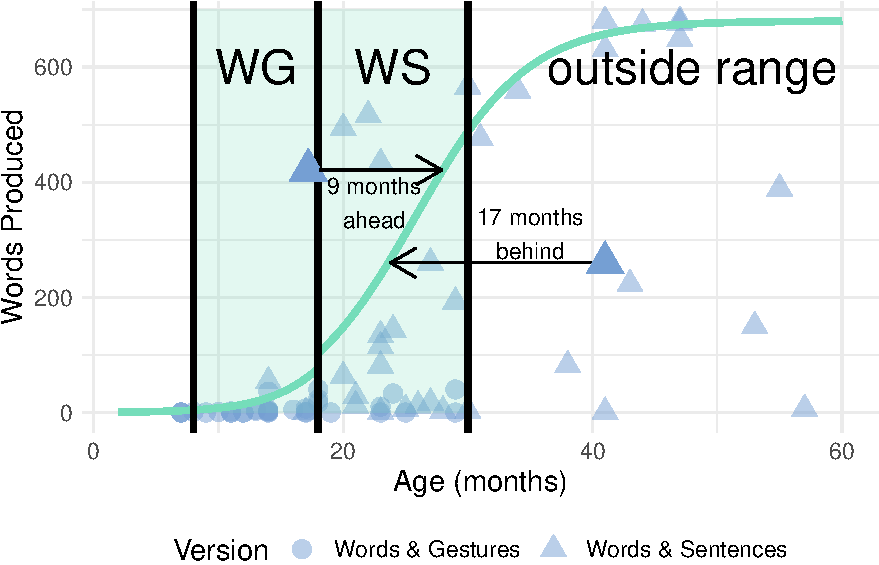
\includegraphics{VI_CDI_manuscript_files/figure-latex/growth-curve-illustration-1.pdf}
\caption{\label{fig:growth-curve-illustration}Visual representation of the months-difference calculation. Shaded region shows the age range covered by the Wordbank norms. Teal line depicts the logistic growth curves constructed from the Wordbank 50th percentile data. Each point represents a blind child's productive vocabulary score from Words and Gestures (circles) or Words and Sentences (triangles); two of these points are enlarged for illustration. To calculate months-difference, we substract the child's chronological age from their expected age (based on vocabulary). In this visualization, months-difference is the x-axis distance between the point and the curve (negative values right of curve, positive are left).}
\end{figure}

Applying this approach to each child, we observe wide variability; vocabulary differences for blind children range from 11 months ahead to 44.50 months behind; see Figure \ref{fig:density-plot}. A Wilcoxon 1-sample test on the data reveals that blind children's vocabulary difference significantly differed from 0 (0 would indicate no difference in vocabulary distribution of blind children from the 50th percentile of sighted children). Blind children had a mean vocabulary delay of 7.20 months (SD: 10). That said, 19\% of our sample was ahead of the sighted 50th percentile norm. That is, rather than all of the blind children being behind the sighted 50th percentile (as would be the case if missing vision led to a pervasive, consistent delay in early word production), or blind children being indistinguishable from sighted peers in vocabulary size (which would have been manifest as roughly 50\% of blind children with delayed and 50\% with advanced vocabulary) we see an intermediary effect: roughly half a year delay on average, with about 20\% of the sample showing a vocabulary advantage over the average for sighted peers.

\begin{figure}
\centering
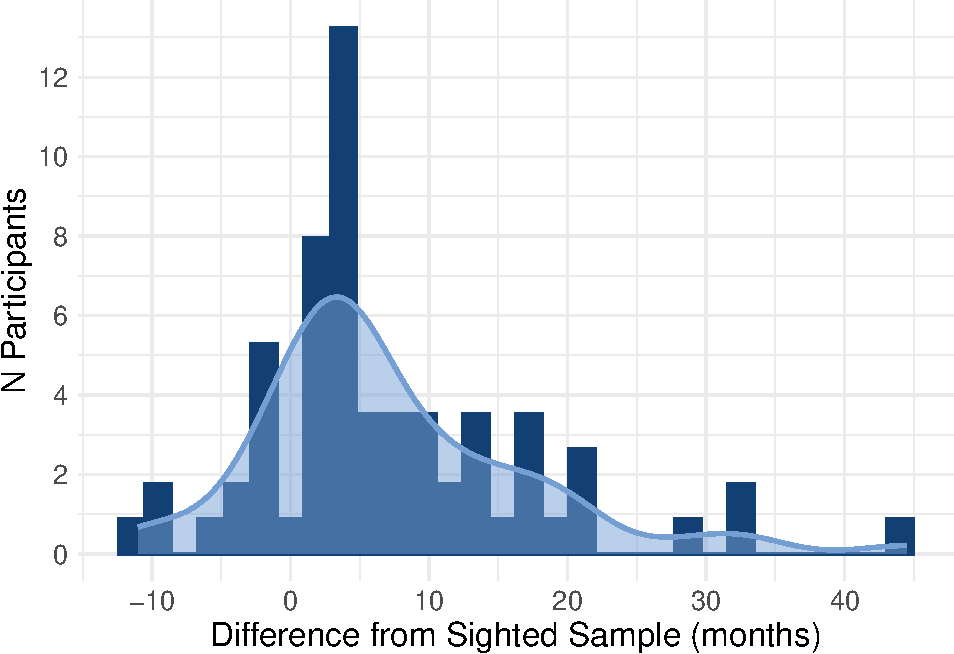
\includegraphics{VI_CDI_manuscript_files/figure-latex/density-plot-1.pdf}
\caption{\label{fig:density-plot}Histogram with overlaid density plot of blind sample's vocabulary difference relative to Wordbank norms. Positive values indicate delay, while negative values represent scores that are ahead of the 50th percentile curve from sighted participants.}
\end{figure}

\hypertarget{exploring-variability}{%
\subsubsection{Exploring Variability}\label{exploring-variability}}

\begin{figure}
\centering
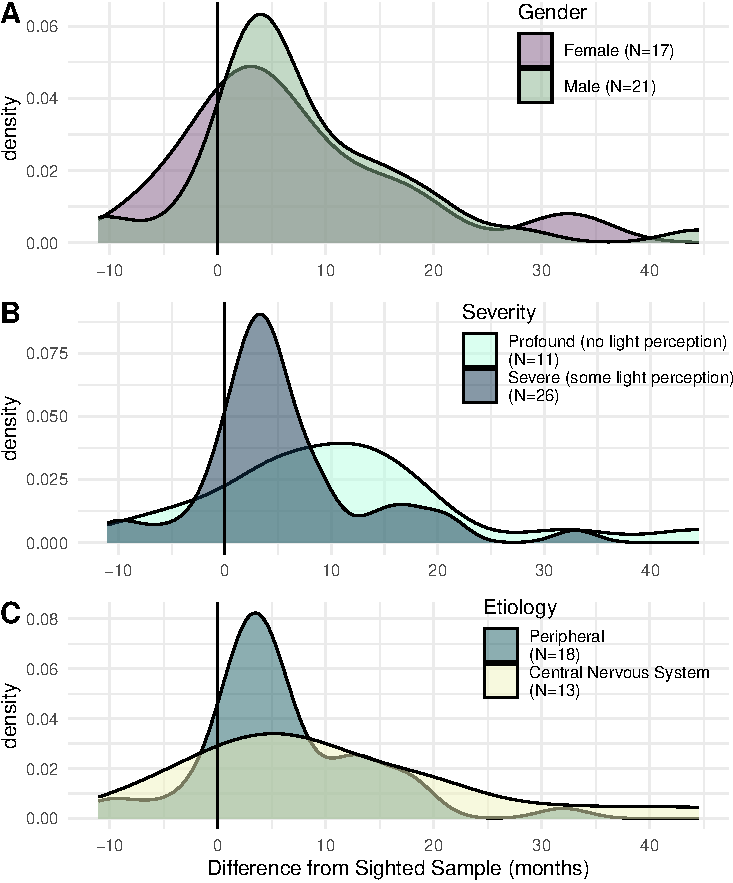
\includegraphics{VI_CDI_manuscript_files/figure-latex/splitting-tests-1.pdf}
\caption{\label{fig:splitting-tests}Density plot dividing the sample by gender (A), severity (B), and etiology (C).}
\end{figure}

To better understand the wide range of vocabulary outcomes, we conducted exploratory analyses aimed at identifying which factors might lead to age-appropriate vocabulary versus delay. We divide our blind sample along several child-level characteristics (gender, degree of vision impairment, and etiology) noted in prior work (e.g. Greenaway \& Dale, 2017; Sakkalou et al., 2021) and compare the distribution of vocabulary differences via Wilcoxon tests; see Figure \ref{fig:splitting-tests}. Splitting the sample by gender (N\textsubscript{male}=21, N\textsubscript{female}=17), boys were numerically roughly two months further delayed than girls; this difference was not statistically significant (Mean\textsubscript{male} delay = 8.27 months vs.~Mean\textsubscript{female} delay = 6.64 months; W = 145.50, \emph{p} = .656). In terms of severity of visual impairment within the severe-to-profound range in our sample, the delay in children with some light perception was numerically about 7 months smaller than in children with no light perception, though again this did not reach statistical significance (some light perception; N\textsubscript{severe}=26; Mean\textsubscript{severe} delay = 5.07 months; no light perception, N\textsubscript{profound}=11; Mean\textsubscript{profound} delay =12.44 months; W = 573.50, \emph{p} = .119). Lastly, we divided by etiology and again found a numerical but not statistically significant difference (W = 527, \emph{p} = .287): children with central nervous system diagnoses (optic nerve hypoplasia or CVI) had a roughly 8 month greater vocabulary delay than children with peripheral diagnoses (N\textsubscript{central}=13; Mean\textsubscript{central} delay =12.07 months; N\textsubscript{peripheral}=18; Mean\textsubscript{peripheral} delay =3.92 months). We note that there was no particular selection for these characteristics within our eligibility criteria, and thus some of these comparisons are on unbalanced samples and we are likely underpowered to detect differences along these dimensions.

\hypertarget{does-the-delay-lessen-across-age}{%
\subsubsection{Does the delay lessen across age?}\label{does-the-delay-lessen-across-age}}

We next measured whether the delay in vocabulary stayed constant across age. We conducted a linear mixed effect model with a fixed effect of age and a random effect of participant, given that for 14 participants, we have longitudinal administrations of the CDI. If delay were constant, we would not expect it to change as children age. Instead, we found a significant effect of age, such that for each month increase in age, vocabulary delay increased by 2.07 weeks (F(1) = 38.72, \emph{p} \textless{} .001); see Figure \ref{fig:longitudinal-plot}.

\begin{figure}
\centering
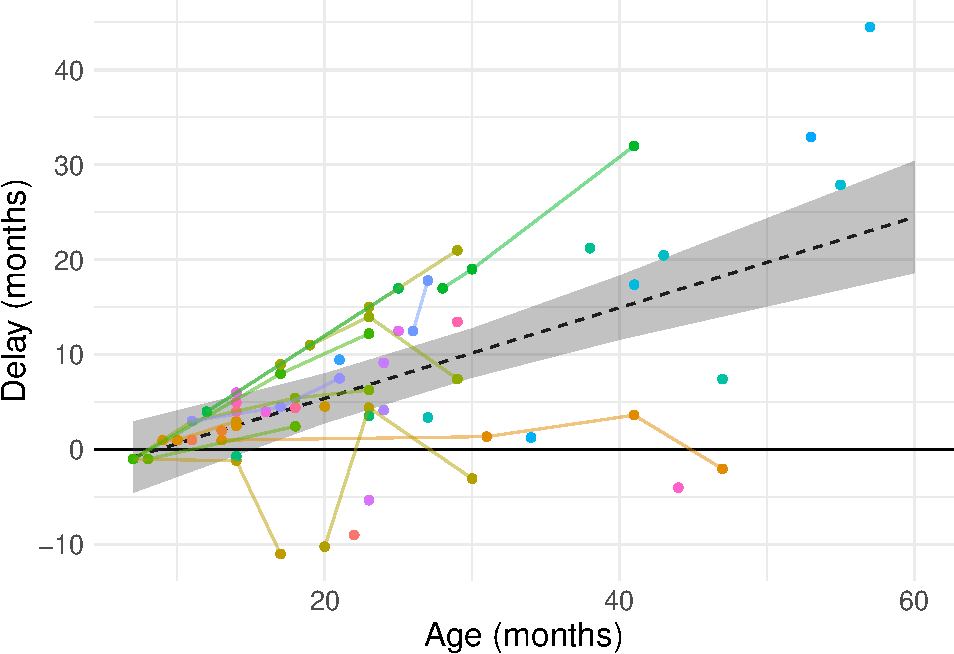
\includegraphics{VI_CDI_manuscript_files/figure-latex/longitudinal-plot-1.pdf}
\caption{\label{fig:longitudinal-plot}Vocabulary delay in blind children plotted as a function of age. Raw data are plotted in color. Each dot represents one CDI administration. When participants have multiple administrations of the CDI, lines connect datapoints from the same participant. Black dashed line represents the model estimate with standard error: Vocabulary Delay \textasciitilde{} Age + (1\textbar Participant).}
\end{figure}

\hypertarget{do-blind-children-and-sighted-children-have-a-similar-vocabulary-composition}{%
\subsection{Do blind children and sighted children have a similar vocabulary composition?}\label{do-blind-children-and-sighted-children-have-a-similar-vocabulary-composition}}

We next investigated the composition of blind children's early words. Given the disparities between the vocabulary production of blind vs.~sighted children, we compared blind participants to a vocabulary-size-matched group of sighted children from Wordbank. We matched each blind child in our sample to a unique sighted participant from Wordbank. Sighted matches were selected to have the same number of words produced on the same form (WG vs.~WS) and to be as close as possible in age to the blind child; beyond this matching they were selected at random\footnote{To ensure that results are not due to the specific blind-sighted pairings, for each blind participant who has multiple possible sighted matches available in Wordbank (N=36/37), we randomly re-assigned matches and re-ran analyses. We find that re-assigning sighted matches does not change the results of our composition comparisons.
}. Consequently, our samples for the vocabulary composition analysis are equivalent in vocabulary production but differ slightly in age (sighted sample on average 4.70 months younger, \emph{p} = .238 by Wilcoxon test); see Figure \ref{fig:vocab-match-demo}.

\begin{figure}
\centering
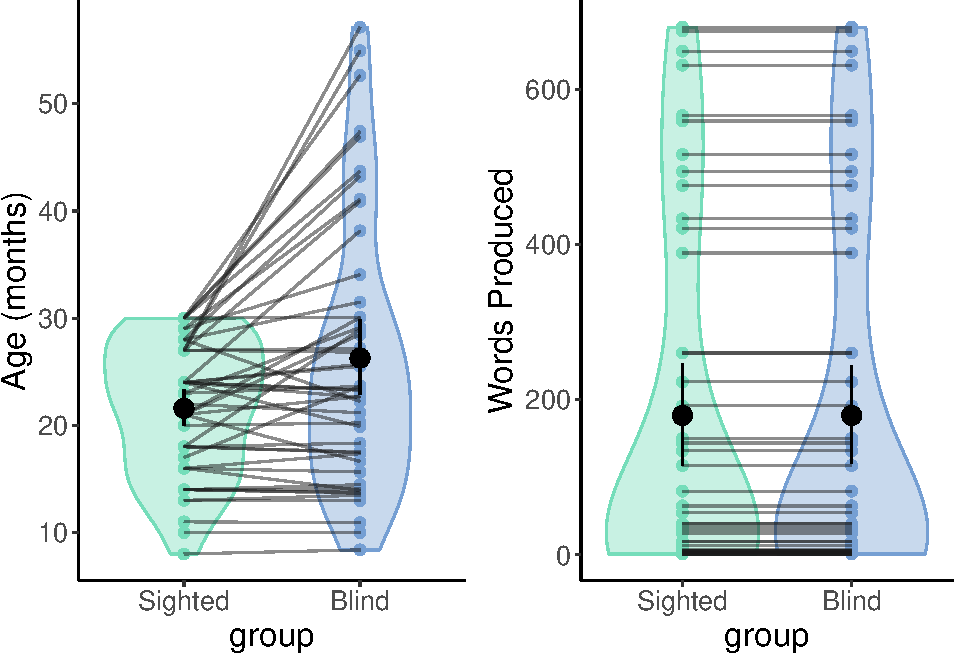
\includegraphics{VI_CDI_manuscript_files/figure-latex/vocab-match-demo-1.pdf}
\caption{\label{fig:vocab-match-demo}Violin plots for age (left) and vocabulary size (right) for blind participants and their vocabulary size matched sighted peers, from Wordbank. Each dot represents one participant. Given that participants are matched exactly on vocabulary, the vocabulary scores on the right panel are identical for blind and sighted participants.}
\end{figure}

We then compared the words that blind and sighted children with equivalent vocabulary size produced. Children producing 0 words were excluded from this analysis (N=3). In order to capture potential phonological, morphosyntactic, and semantic differences in the early lexicon, we compared vocabularies along six dimensions: word length, part of speech, semantic category, concreteness, child-body-object interaction rating (interactiveness), and perceptual modality, operationalized below.

\textbf{Word length} was computed as number of syllables in each word. \textbf{Part of speech} (adjectives, adverbs, function words, interjections, nouns, onomatopoeia, and verbs) and \textbf{semantic category}\footnote{Not all categories from Words and Sentences appear on Words and Gestures. Additionally, some of the "semantic categories" could also be considered parts of speech. The word-level breakdown of each of these categories can be found on our OSF page.} (action words, animals, body parts, clothing, connecting words, descriptive words, food and drink, furniture and rooms, games and routines, helping verbs, household, locations, outside, people, places, pronouns, quantifiers, question words, sounds, time words, toys, and vehicles) subdivisions were taken from the categories on the CDI. For \textbf{concreteness}, we used the Brysbaert Concreteness ratings (Brysbaert, Warriner, \& Kuperman, 2014), which asked sighted adult participants to rate words from 1 (Abstract - language based) to 5 (Concrete - experience based); 30 words were excluded from this analysis due to not having a concreteness rating. \textbf{Interactiveness} ratings were taken from the child-body-object interactiveness ratings from Muraki et al. (2022). These are 1-7 ratings by parents of school-aged children of how easily children can physically interact with each of the words. 30 words were excluded from this analysis due to not having a rating. Lastly, \textbf{perceptual modality} was determined by the Lancaster Sensorimotor Norms (Lynott, Connell, Brysbaert, Brand, \& Carney, 2020), taken from a large sample of sighted adults, who were asked to rate: ``To what extent do you experience WORD by {[}hearing, smelling, tasting, seeing, etc.{]}?'' Each word was rated 0-5 for each modality, and the modality which received the highest rating is used here for the perceptual modality of the word.

To compare words across each of these dimensions, we used profile analyses and Wilcoxon tests, depending on the type of variable. For semantic category, perceptual modality, and part of speech, we compared counts of each word type across groups using profile analysis (Bulut \& Desjardins, 2020). For concreteness and word length, we ran Wilcoxon tests. Given that we conducted multiple exploratory comparisons (six total, one per dimension), the Bonferroni-corrected threshold for significance is 0.0083.

\begin{figure}
\centering
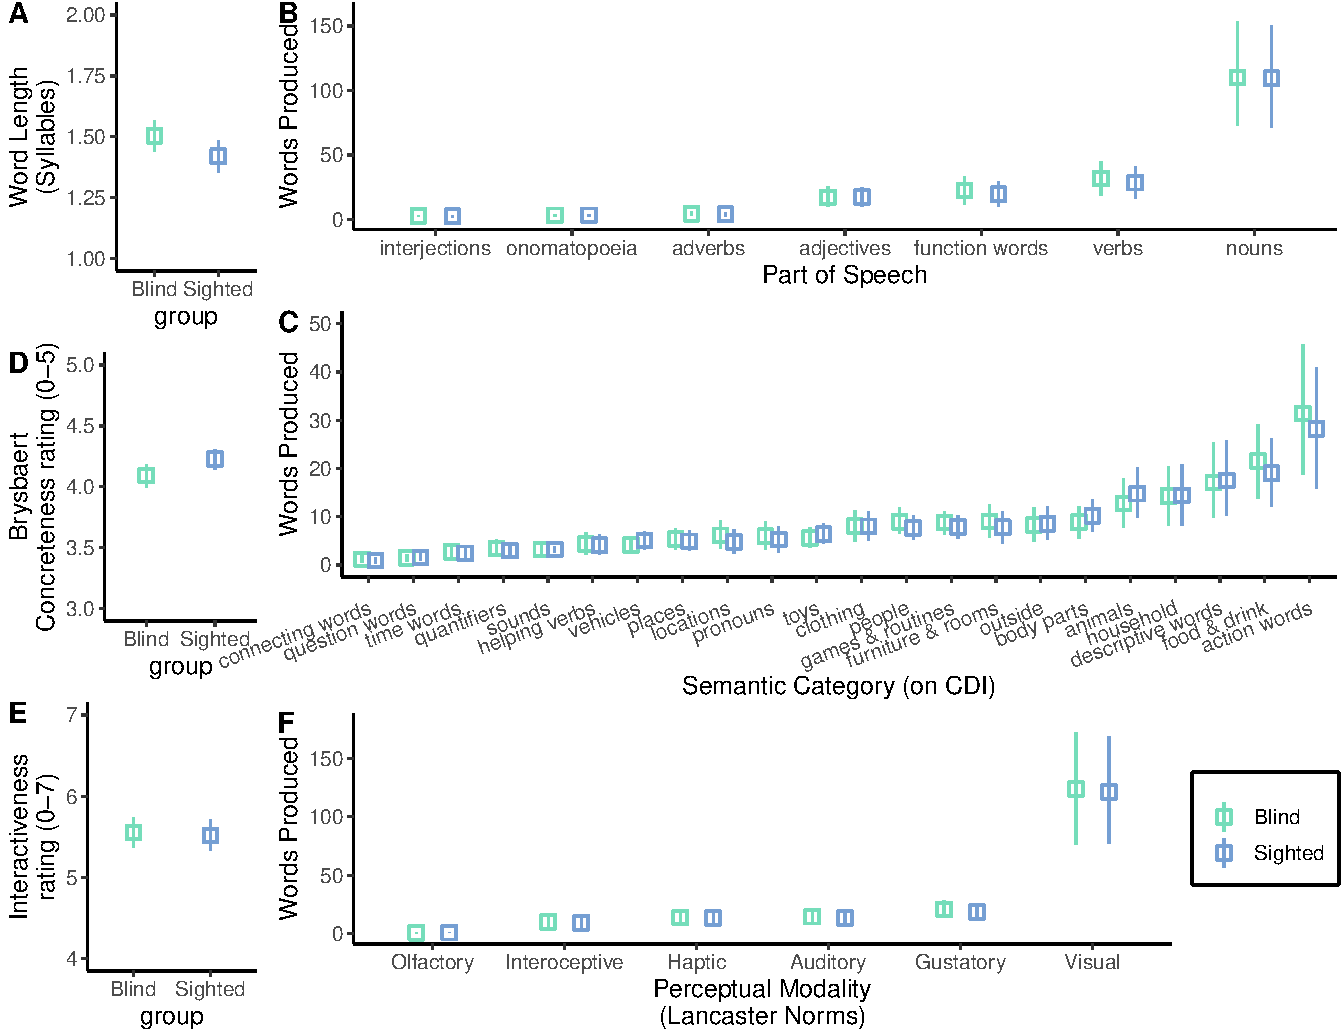
\includegraphics{VI_CDI_manuscript_files/figure-latex/vocab-comparison-1.pdf}
\caption{\label{fig:vocab-comparison}Comparisons of blind and sighted children's vocabulary across 6 dimensions. Whiskers represent 95\% CIs around the mean. \textbf{A}: Mean length (syllables) for sighted vs.~blind participants. \textbf{B}: Mean N of words produced by blind and sighted children from each part of speech on CDI. \textbf{C}: Mean N of words produced by blind and sighted children from each semantic category on CDI. \textbf{D}: Mean concreteness rating 1 (abstract) -- 5 (concrete) for sighted vs.~blind participants. \textbf{E}: Mean child-body-object interaction rating 1 (not interactive) -- 7 (highly interactive) for sighted vs.~blind participants. \textbf{F}: Mean N of words produced by blind and sighted children for each perceptual modality (modality with highest perceptual rating on Lancaster Sensorimotor Norms). Note the truncated y axis for D and E.}
\end{figure}

None of the comparisons reached this corrected threshold for significance. Blind and sighted children's early vocabularies did not significantly differ in word length (W =434, \emph{Z} = -1.58, \emph{p} = .115), part of speech (F = 1.66, \emph{p} = .144), semantic category (F = 1.89, \emph{p} = .033), concreteness (W =208, \emph{Z} = -1.96, \emph{p} = .050), interactiveness (W =639.50, \emph{Z} = -0.09, \emph{p} = .928), or perceptual modality (F = 2.26, \emph{p} = .058). See Figure \ref{fig:vocab-comparison} for vocabulary comparisons. Descriptively, both blind and sighted children's words tended to be short (Means: 1.46 and 1.52 syllables, respectively) and highly concrete (Means: 4.14 and 4.08 out of 5, respectively). The words that blind and sighted children produced tended to be rated as easy for children to interact with (Means: 5.50 and 5.50 out of 7, respectively). In both groups, nouns were the most common part of speech, and visual words comprised the overwhelming majority of children's early vocabulary.

\begin{figure}
\centering
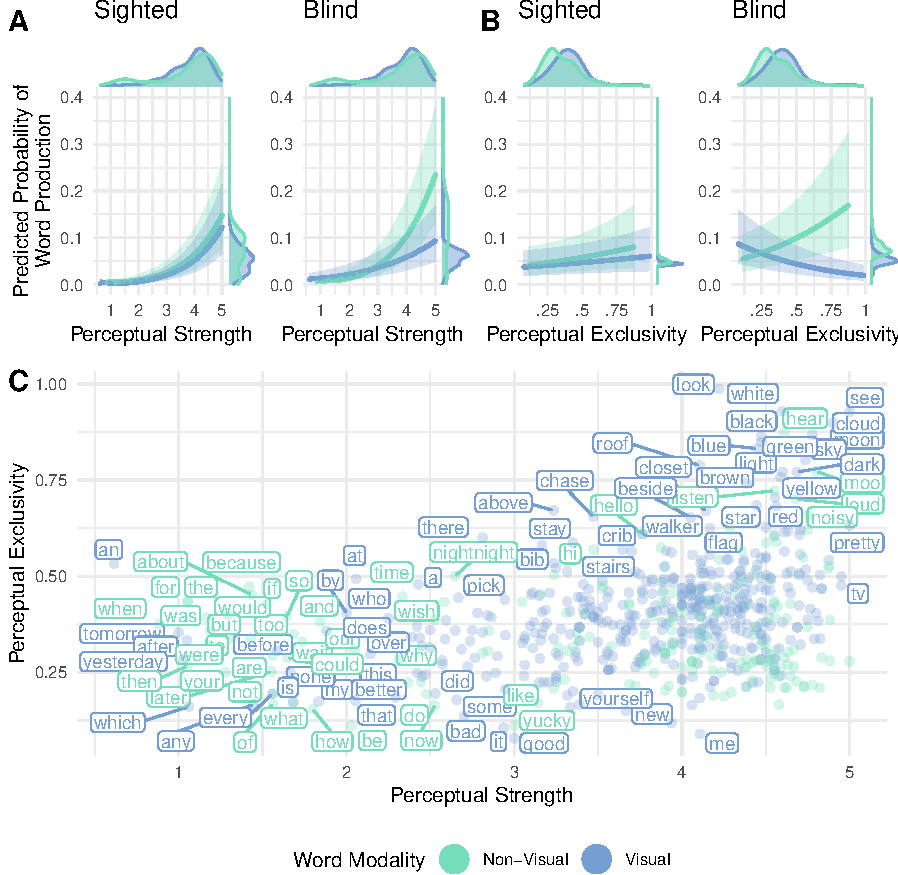
\includegraphics{VI_CDI_manuscript_files/figure-latex/visualornot-1.pdf}
\caption{\label{fig:visualornot}Visualization of the significant 3-way interaction between \textbf{A} Modality (visual/non-visual), Perceptual Strength (0-5), and Group (blind/sighted) and \textbf{B} Modality, Perceptual Exclusivity (0-1), and Group in predicting probability of word production (see text for model details). Y-axis shows the model-predicted probability of word production, with 95\% confidence interval; distribution of predicted probability (of individual words) shown in margins. The x-axis shows perceptual property (perceptual strength in A, perceptual exclusivity in B); distribution of words' varying ratings shown in margins. \textbf{C}: Perceptual properties of visual and non-visual on the CDI -- perceptual strength on the x-axis and perceptual exclusivity on the y-axis. Some individual words are labeled for illustrative purposes.}
\end{figure}

\hypertarget{how-do-perceptual-characteristics-of-words-affect-learnability}{%
\subsection{How do perceptual characteristics of words affect learnability?}\label{how-do-perceptual-characteristics-of-words-affect-learnability}}

On one hand, it was somewhat surprising to find such striking parallels in blind and sighted children's vocabulary, particularly the dominance of ``visual'' words, given that blind children lack visual access to the words' referents. Notably, prior work e.g.~Landau \& Gleitman (1985) suggests their blind subject Kelli also produced highly visual words, though word modality distributions over the vocabulary was not something they explored. More germanely, it's worth noting that words the Lancaster Sensorimotor norms classify as visual are often perceptible through other modalities. For example, while ``playground'' is classified as a visual word on the Lancaster Sensorimotor Norms, playgrounds can also be experienced through touch, sound, smell, or even taste. This raises the possibility that although blind and sighted children's vocabularies contain similar amounts of visual words, the visual words that blind children produce may be qualitatively different from the visual words that sighted children produce. To explore this, we next compared blind and sighted children's likelihood of producing visual words (i.e., words whose highest perceptual ratings were visual) and non-visual words (i.e., words whose highest perceptual ratings were auditory, tactile, olfactory, interoceptive, or gustatory), based on the perceptual strength of each word and its perceptual exclusivity (operationalized below). Words that did not appear on a child's instrument (e.g., lawnmower does not appear on the Words and Gestures CDI) were excluded for those children.

To do this, we constructed two logistic mixed effect models that predicted the log likelihood of a word being produced as a function of the three way interaction between the word's perceptual modality (visual or non-visual)\footnote{Given the large proportion of visual words and relative sparsity of other modalities in children's vocabulary, we grouped auditory, tactile, haptic, interoceptive, olfactory, and gustatory words into a "non-visual" category for the purpose of this analysis.}, group (blind or sighted), and either the word's perceptual strength (highest perceptual strength rating across all modalities, rated 1-5) or the word's perceptual exclusivity (expressed as a proportion from 0-1 calculated as the range of the ratings of all modalities divided by the sum of the ratings of all modalities. 0 = experienced equally in all modalities, 1 = experienced exclusively through a single modality); model formulae are below. Each model also included a random effect of child since each child contributes multiple datapoints (one for each word on the CDI), as well as a random effect for word given that there is an observation for each word for each participant, and the likelihood of word-level variance being non-random (though not of interest for the present analysis). Thus, we fit two models as follows:\\
\textbf{Perceptual Strength Model:} \(Word\ Production \sim Perceptual\ Strength * Perceptual\ Modality * Group + (1|Participant) + (1|Word)\)\\
\textbf{Perceptual Exclusivity Model:} \(Word\ Production \sim Perceptual\ Exclusivity * Perceptual\ Modality * Group + (1|Participant) + (1|Word)\)

For the perceptual strength model (Table \ref{tab:ps-table}), we found a significant main effect of perceptual strength (\(\beta\) = 0.90, \emph{p} \textless{} .001). Overall, the groups did not differ in likelihood of producing words (\(\beta\) = 0.22, \emph{p} = .844), and the effect of perceptual strength did not differ by modality (\(\beta\) = -0.37, \emph{p} = .573). This pattern of main effects was qualified by a significant interaction between group and perceptual strength such that the effect of perceptual strength was stronger for the blind group than the sighted group (\(\beta\) = 0.15, \emph{p} = .041), as well as a significant interaction between group and modality, such that blind children were significantly less likely to produce visual words than non-visual words (\(\beta\) = 1.82, \emph{p} \textless{} .001). Finally, there was a significant three-way interaction between modality, perceptual strength, and group, such that for sighted children, there was a similar effect of perceptual strength for visual and non-visual words. For blind children however, the effect of perceptual strength was much stronger for non-visual words than visual words (\(\beta\) = -0.56, \emph{p} \textless{} .001). This suggests that for sighted children, higher perceptual strength boosts the likelihood of word production across perceptual modalities. In contrast, for blind children, the effect of visual association strength was much weaker than the effect of perceptual strength with other modalities (sound, touch, etc.). See Figure \ref{fig:visualornot}.

\begin{table}[H]

\caption{\label{tab:ps-table}Logistic regression estimates for the perceptual strength model (see formula in main text). Reference level for Modality is non-visual, and reference level for Group is sighted. Parentheticals indicate what is being compared to reference level.}
\centering
\begin{tabular}[t]{l|l|l}
\hline
Variable & Beta [95\% CI] & p value\\
\hline
(Intercept) & -5.71 [-7.49, -3.94] & 0.000***\\
\hline
Modality (visual) & -0.37 [-1.64, 0.91] & 0.573\\
\hline
Perceptual Strength & 0.90 [0.66, 1.14] & 0.000***\\
\hline
Group (blind) & 0.22 [-1.99, 2.43] & 0.844\\
\hline
Modality (visual):Perceptual Strength & 0.02 [-0.31, 0.35] & 0.891\\
\hline
Modality (visual):Group (blind) & 1.82 [1.05, 2.59] & 0.000***\\
\hline
Perceptual Strength:Group (blind) & 0.15 [0.01, 0.30] & 0.041*\\
\hline
Modality (visual):Perceptual Strength:Group (blind) & -0.56 [-0.75, -0.36] & 0.000***\\
\hline
\end{tabular}
\end{table}

For the perceptual exclusivity model (Table \ref{tab:excl-table}), we again found that the groups did not differ in overall likelihood of producing words (\(\beta\) = 0.66, \emph{p} = .552). The main effect of perceptual exclusivity was not significant (\(\beta\) = 1.10, \emph{p} = .302), and did not differ by group (\(\beta\) = 0.37, \emph{p} = .494). Here too, this pattern of main effects was qualified by a significant interaction between group and modality, such that blind children were significantly less likely to produce visual words (\(\beta\) = 0.65, \emph{p} = .010). Finally, we again observed a three-way interaction, here between modality, perceptual exclusivity, and group, such that for the sighted group, words that were more unimodal were more likely to be produced for both visual and non-visual words. By contrast, for the blind group, non-visual words that were more unimodal were more likely to be produced, but visual words that were more unimodal were \emph{less} likely to be produced (\(\beta\) = -2.49, \emph{p} \textless{} .001). This interaction suggests that for blind children, visual words that could only be experienced through one domain (vision) were less likely to be produced. For the \emph{non}-visual words for blind children, and for all words for sighted children, there was no significant effect of perceptual exclusivity.

\begin{table}[H]

\caption{\label{tab:excl-table}Logistic regression estimates for the perceptual exclusivity model (see formula in main text). Reference level for Modality is non-visual, and reference level for Group is sighted. Parentheticals indicate what is being compared to reference level.}
\centering
\begin{tabular}[t]{l|l|l}
\hline
Variable & Beta [95\% CI] & p value\\
\hline
(Intercept) & -2.76 [-4.46, -1.05] & 0.002**\\
\hline
Modality (visual) & 0.12 [-0.83, 1.08] & 0.802\\
\hline
Perceptual Exclusivity & 1.10 [-0.99, 3.20] & 0.302\\
\hline
Group (blind) & 0.66 [-1.52, 2.85] & 0.552\\
\hline
Modality (visual):Perceptual Exclusivity & -0.87 [-3.32, 1.59] & 0.490\\
\hline
Modality (visual):Group (blind) & 0.65 [0.15, 1.14] & 0.010*\\
\hline
Perceptual Exclusivity:Group (blind) & 0.37 [-0.69, 1.42] & 0.494\\
\hline
Modality (visual):Perceptual Exclusivity:Group (blind) & -2.49 [-3.75, -1.23] & 0.000***\\
\hline
\end{tabular}
\end{table}

\hypertarget{discussion}{%
\section{Discussion}\label{discussion}}

This study compared the early vocabularies of blind and sighted children to better understand the influence of vision on acquiring a lexicon. We found that while blind children in our sample showed vocabulary delays, there were remarkable similarities between the vocabulary composition of blind and sighted children. These results suggest that while visual perception appears to support vocabulary acquisition, it does not seem to determine the overall composition of the early lexicon. We further found that the likelihood of word production was predicted by children's access to words through one vs.~multiple modalities.

While the absence of vision does seem to result in vocabulary delays for most children (in our sample, roughly half a year delay on average, with \textasciitilde20\% of blind children ahead of the 50th percentile of sighted children), the exact mechanism by which vision influences vocabulary growth remains unclear. Referential transparency alone seems unlikely: when blind children learn words, they learn a similar number of ``visual'' words as sighted children. Future work measuring social, motor, and cognitive development alongside vocabulary in blind children may illuminate skills that support word learning. Differences in language input to blind children could also explain the wide variability in language outcomes. By hypothesis, associations between language input and vocabulary development might even be stronger in blind children, given that language may be blind children's source of ``visual'' information about the world (Campbell \& Bergelson, 2022b).

While we only included participants without diagnosed cognitive or developmental delays, some participants had vocabulary sizes that fell on the extremes of the distribution; this might flag the need for early intervention services to support cognitive and linguistic development. Given that many early childhood cognitive assessments are not accessible for children with visual impairments (e.g., WPPSI-IV, DAS-II; Bayley, but cf.~Dale et al., 2014), monitoring productive vocabulary growth could provide insight into blind children's cognitive development, though we caution that such an approach has yet to be validated.

Although evidence from blind adults and older children suggests that language skills improve (Landau \& Gleitman, 1985; Loiotile et al., 2020; Röder et al., 2003), we did not see evidence that vocabulary delays lessen in our age group. In fact, older children in our sample have larger delays. This could be a floor effect: the \emph{possible} size of the delay increases over time, such that 12-month-olds cannot be 18 months delayed, but 30-month-olds can. That said, if blind children, after an initial delay, learn words at the same rate as the sighted peers we would expect to see a constant delay; we saw an increasing one. This bumps the question downstream: if blind children eventually catch up to sighted peers, when and how does this happen?

One possibility is that blind children initially struggle with word learning. The first words in blind children's vocabulary might be hard-earned. Vision might provide an easier or more efficient way for sighted children to connect referents to objects in their environment. Perhaps after blind children build their initial lexicon, they can leverage linguistic structure more effectively, through processes like syntactic bootstrapping (e.g., Babineau, de Carvalho, Trueswell, \& Christophe, 2021; Gleitman, 1990). Evaluating this hypothesis awaits further work.

Turning to vocabulary \emph{content}, blind and sighted children's lexicons were overwhelmingly similar: they were characterized by noun dominance, short, concrete, physically interactive words, and common topics (Frank, Braginsky, Yurovsky, \& Marchman, 2021). Summarizing, blind children learn largely the same set of early words as sighted children. And while we found that the vocabularies of both sighted and blind children were dominated by ``visual'' words, the bulk of the words on the CDI (and indeed, the English language, Winter, Perlman, \& Majid, 2018) are rated by sighted adults as primarily associated with visual experience. In addition, our approach to measuring visualness implicitly assumes that ratings from sighted adults are valid for blind children; in ongoing work, we are creating new norms from blind adults to further explore how these ratings may vary by sensory experience.

That said, we found that learnability of visual words differed based on words' finer-grained perceptual properties. For blind children, higher perceptual exclusivity (less multimodality) predicted \emph{lower} likelihood of production for visual words (but not non-visual words). For sighted children, perceptual exclusivity did not effect production of either word type. Relatedly, for blind children, higher perceptual strength ratings predicted greater likelihood of word production for non-visual words, but lacked this strong relationship for visual words. Constrastingly, in sighted children, higher perceptual strength predicted greater production likelihood of all words. These exploratory findings suggest that visual words like \emph{light} (highly visual and unidimensional), are less likely to be produced by blind children relative to ``visual'' words that can be perceived through other modalities (e.g.~\emph{table}). Returning to the earlier literature, these findings help us contextualize prior work such as Landau and Gleitman (1985)'s work with the blind child ``Kelli''. Given, as we show here, that highly and exclusively visual words like ``see'' or ``red'', are less likely to appear in blind children's early lexicons, it is notable that when they do appear, children demonstrate sophisticated semantic understanding (Landau \& Gleitman, 1985). That said, our work does not run counter to this prior work: it is both the case that some blind children produce more unimodal highly visual words like color terms and that on average across a sample of such children, these words are delayed relative to sighted peers. A deeper understanding of how blind children acquire the meanings of these highly visual words remains an open question.

It is worth acknowledging here that the CDI is a finite list of words, which offers a structured framework for assessing vocabulary development, but may limit its coverage of children's early lexicons. At either end of the distribution (e.g., kids producing 0 words, kids producing all words), there is less room for variability. That said, the words on the CDI were selected explicitly to provide gradation in difficulty, in order to reflect a range of lexical abilities. Additionally, it's highly likely that children---both blind and sighted---are producing words that are not on the CDI's word list; it's further possible that blind children's early words are disproportionately left off of the CDI. Anecdotally, one parent of a blind child in our sample told us that her child says ``gastroenterologist,'' an item certainly not on the CDI. Analyses of naturalistic recordings of blind children's early language (currently ongoing) may help illuminate vocabulary production not captured on the CDI.

As a relatively large-scale study of language development in young blind children, these results are clinically relevant. Chiefly, blind children are at risk of language delays and may benefit from early intervention communication support. While initial delays may resolve (Brambring, 2007), providing young blind children and their caregivers with tools to communicate better may reduce children's frustration in toddlerhood (Manning et al., 2019).

It is worth noting that by design, this study does not capture the full linguistic or diagnostic variability of the blind population. We constrained the sample to young, monolingual, English-speaking blind children with no more than minimal light perception and no cognitive, developmental, or auditory diagnoses. In reality, the population of children with visual impairments encompasses a broad range of perceptual abilities, language backgrounds, and life experiences. Future work could investigate whether these results generalize to more diverse samples or whether variability in language background or diagnosis contributes to differences in vocabulary outcomes.

Many questions remain regarding how vision interacts with children's social and cognitive skills to form the lexicon. What do blind children's early representations of visual words entail? Is the lexicon organized similarly? How do blind children extract visual information from language input to learn more about both language and their environment? Future work on language development in blind children capturing a more holistic view of blind children's skills and environments is needed to further our understand of how perception and language input interact to support children's learning.

\hypertarget{references}{%
\section*{References}\label{references}}
\addcontentsline{toc}{section}{References}

\hypertarget{refs}{}
\begin{CSLReferences}{1}{0}
\leavevmode\vadjust pre{\hypertarget{ref-adolph2015}{}}%
Adolph, K., \& Robinson, S. (2015). Motor {Development}. In \emph{Cognitive processes} (Vol. 2, pp. 113--157). \url{https://doi.org/10.1002/9781118963418.childpsy204}

\leavevmode\vadjust pre{\hypertarget{ref-andersen1984}{}}%
Andersen, E. S., Dunlea, A., \& Kekelis, L. S. (1984). Blind {Children}'s {Language}: {Resolving Some Differences}. \emph{Journal of Child Language}, \emph{11}(3), 645--664. \url{https://doi.org/10.1017/s0305000900006000}

\leavevmode\vadjust pre{\hypertarget{ref-babineau2021}{}}%
Babineau, M., de Carvalho, A., Trueswell, J., \& Christophe, A. (2021). Familiar words can serve as a semantic seed for syntactic bootstrapping. \emph{Developmental Science}, \emph{24}(1), e13010. \url{https://doi.org/10.1111/desc.13010}

\leavevmode\vadjust pre{\hypertarget{ref-berthier2006}{}}%
Berthier, N. E., \& Keen, R. (2006). Development of reaching in infancy. \emph{Experimental Brain Research}, \emph{169}(4), 507--518. \url{https://doi.org/10.1007/s00221-005-0169-9}

\leavevmode\vadjust pre{\hypertarget{ref-bigelow1986}{}}%
Bigelow, A. (1986). The development of reaching in blind children. \emph{British Journal of Developmental Psychology}, \emph{4}(4), 355--366. \url{https://doi.org/10.1111/j.2044-835X.1986.tb01031.x}

\leavevmode\vadjust pre{\hypertarget{ref-bigelow1987}{}}%
Bigelow, A. (1987). Early words of blind children. \emph{Journal of Child Language}, \emph{14}(1), 47--56. \url{https://doi.org/10.1017/S0305000900012721}

\leavevmode\vadjust pre{\hypertarget{ref-bigelow2003}{}}%
Bigelow, A. (2003). Development of joint attention in blind infants. \emph{Development and Psychopathology}, \emph{15}, 259--275. \url{https://doi.org/10.1017/S0954579403000142}

\leavevmode\vadjust pre{\hypertarget{ref-bottini2022}{}}%
Bottini, R., Morucci, P., D'Urso, A., Collignon, O., \& Crepaldi, D. (2022). The concreteness advantage in lexical decision does not depend on perceptual simulations. \emph{Journal of Experimental Psychology: General}, \emph{151}(3), 731--738. \url{https://doi.org/10.1037/xge0001090}

\leavevmode\vadjust pre{\hypertarget{ref-brambring2007}{}}%
Brambring, M. (2007). Divergent {Development} of {Verbal Skills} in {Children} who are {Blind} or {Sighted}. \emph{Journal of Visual Impairment \& Blindness}, \emph{101}(12), 749--762. \url{https://doi.org/10.1177/0145482X0710101205}

\leavevmode\vadjust pre{\hypertarget{ref-brooks2008}{}}%
Brooks, R., \& Meltzoff, A. N. (2008). Infant gaze following and pointing predict accelerated vocabulary growth through two years of age: A longitudinal, growth curve modeling study*. \emph{Journal of Child Language}, \emph{35}(1), 207--220. \url{https://doi.org/10.1017/S030500090700829X}

\leavevmode\vadjust pre{\hypertarget{ref-brysbaert2014}{}}%
Brysbaert, M., Warriner, A. B., \& Kuperman, V. (2014). Concreteness ratings for 40 thousand generally known {English} word lemmas. \emph{Behavior Research Methods}, \emph{46}(3), 904--911. \url{https://doi.org/10.3758/s13428-013-0403-5}

\leavevmode\vadjust pre{\hypertarget{ref-bulut2020}{}}%
Bulut, O., \& Desjardins, C. D. (2020). \emph{Profile {Analysis} of {Multivariate Data}: {A Brief Introduction} to the {profileR Package}}. {PsyArXiv}. \url{https://doi.org/10.31234/osf.io/sgy8m}

\leavevmode\vadjust pre{\hypertarget{ref-campbell2022b}{}}%
Campbell, E. E., \& Bergelson, E. (2022a). Characterizing {North Carolina}'s {Deaf} and {Hard} of {Hearing Infants} and {Toddlers}: {Predictors} of {Vocabulary}, {Diagnosis}, and {Intervention}. \emph{Journal of Speech, Language, and Hearing Research}, \emph{65}(5), 1894--1905. \url{https://doi.org/10.1044/2022_JSLHR-21-00245}

\leavevmode\vadjust pre{\hypertarget{ref-campbell2022a}{}}%
Campbell, E. E., \& Bergelson, E. (2022b). Making sense of sensory language: {Acquisition} of sensory knowledge by individuals with congenital sensory impairments. \emph{Neuropsychologia}, \emph{174}, 108320. \url{https://doi.org/10.1016/j.neuropsychologia.2022.108320}

\leavevmode\vadjust pre{\hypertarget{ref-carpenter1998}{}}%
Carpenter, M., Nagell, K., Tomasello, M., Butterworth, G., \& Moore, C. (1998). Social {Cognition}, {Joint Attention}, and {Communicative Competence} from 9 to 15 {Months} of {Age}. \emph{Monographs of the Society for Research in Child Development}, \emph{63}(4), i--174. \url{https://doi.org/10.2307/1166214}

\leavevmode\vadjust pre{\hypertarget{ref-clerkin2017}{}}%
Clerkin, E. M., Hart, E., Rehg, J. M., Yu, C., \& Smith, L. B. (2017). Real-world visual statistics and infants' first-learned object names. \emph{Philosophical Transactions of the Royal Society B: Biological Sciences}, \emph{372}(1711), 20160055. \url{https://doi.org/10.1098/rstb.2016.0055}

\leavevmode\vadjust pre{\hypertarget{ref-clerkin2022}{}}%
Clerkin, E. M., \& Smith, L. B. (2022). Real-world statistics at two timescales and a mechanism for infant learning of object names. \emph{Proceedings of the National Academy of Sciences}, \emph{119}(18), e2123239119. \url{https://doi.org/10.1073/pnas.2123239119}

\leavevmode\vadjust pre{\hypertarget{ref-clifton1993}{}}%
Clifton, R. K., Muir, D. W., Ashmead, D. H., \& Clarkson, M. G. (1993). \href{https://www.ncbi.nlm.nih.gov/pubmed/8404258}{Is visually guided reaching in early infancy a myth?} \emph{Child Development}, \emph{64}(4), 1099--1110.

\leavevmode\vadjust pre{\hypertarget{ref-colonnesi2010}{}}%
Colonnesi, C., Stams, G. J. J. M., Koster, I., \& Noom, M. J. (2010). The relation between pointing and language development: {A} meta-analysis. \emph{Developmental Review}, \emph{30}(4), 352--366. \url{https://doi.org/10.1016/j.dr.2010.10.001}

\leavevmode\vadjust pre{\hypertarget{ref-dale2014}{}}%
Dale, N. J., Tadić, V., \& Sonksen, P. (2014). Social communicative variation in 1-3-year-olds with severe visual impairment: {Social} communication in visually impaired 1-3-year-olds. \emph{Child: Care, Health and Development}, \emph{40}(2), 158--164. \url{https://doi.org/10.1111/cch.12065}

\leavevmode\vadjust pre{\hypertarget{ref-demott1972}{}}%
DeMott, R. M. (1972). Verbalism and affective meaning for blind, severely visually impaired, and normally sighted children. \emph{New Outlook for the Blind}, \emph{66}(1), 1--8, 25.

\leavevmode\vadjust pre{\hypertarget{ref-dunlea1989}{}}%
Dunlea, A. (1989). \emph{Vision and the emergence of meaning: {Blind} and sighted children's early language} (pp. xv, 196). {New York, NY, US}: {Cambridge University Press}. \url{https://doi.org/10.1017/CBO9780511519802}

\leavevmode\vadjust pre{\hypertarget{ref-elisa2002}{}}%
Elisa, F., Josée, L., Oreste, F.-G., Claudia, A., Antonella, L., Sabrina, S., \& Giovanni, L. (2002). Gross motor development and reach on sound as critical tools for the development of the blind child. \emph{Brain and Development}, \emph{24}(5), 269--275. \url{https://doi.org/10.1016/S0387-7604(02)00021-9}

\leavevmode\vadjust pre{\hypertarget{ref-fraiberg1977}{}}%
Fraiberg, S., \& Fraiberg, L. (1977). \emph{Insights from the blind: {Comparative} studies of blind and sighted infants}. {New York, NY, USA}: {Basic Books}.

\leavevmode\vadjust pre{\hypertarget{ref-frank2017}{}}%
Frank, M. C., Braginsky, M., Yurovsky, D., \& Marchman, V. A. (2017). Wordbank: An open repository for developmental vocabulary data. \emph{Journal of Child Language}, \emph{44}(3), 677--694. \url{https://doi.org/10.1017/S0305000916000209}

\leavevmode\vadjust pre{\hypertarget{ref-frank2021}{}}%
Frank, M. C., Braginsky, M., Yurovsky, D., \& Marchman, V. A. (2021). \emph{Variability and {Consistency} in {Early Language Learning}: {The Wordbank Project}}. {Cambridge}: {The MIT Press}.

\leavevmode\vadjust pre{\hypertarget{ref-garcia-filion2013}{}}%
Garcia-Filion, P., \& Borchert, M. (2013). Optic {Nerve Hypoplasia Syndrome}: {A Review} of the {Epidemiology} and {Clinical Associations}. \emph{Current Treatment Options in Neurology}, \emph{15}(1), 78--89. \url{https://doi.org/10.1007/s11940-012-0209-2}

\leavevmode\vadjust pre{\hypertarget{ref-gilbert2003}{}}%
Gilbert, C., \& Awan, H. (2003). \href{https://www.ncbi.nlm.nih.gov/pmc/articles/PMC214052}{Blindness in children}. \emph{BMJ : British Medical Journal}, \emph{327}(7418), 760--761.

\leavevmode\vadjust pre{\hypertarget{ref-gleitman1990}{}}%
Gleitman, L. (1990). The {Structural Sources} of {Verb Meanings}. \emph{Language Acquisition}, \emph{1}(1), 3--55. Retrieved from \url{https://www.jstor.org/stable/20011341}

\leavevmode\vadjust pre{\hypertarget{ref-greenaway2017}{}}%
Greenaway, R., \& Dale, N. J. (2017). Congenital {Visual Impairment}. In \emph{Research in {Clinical Pragmatics}}.

\leavevmode\vadjust pre{\hypertarget{ref-harley1963}{}}%
Harley, R. K. (1963). \emph{Verbalism {Among Blind Children}; {An Investigation} and {Analysis}. {American Foundation} for the {Blind Research Series}, {Number} 10}.

\leavevmode\vadjust pre{\hypertarget{ref-heilmann2005}{}}%
Heilmann, J., Weismer, S. E., Evans, J., \& Hollar, C. (2005). Utility of the {MacArthur}\textemdash{{Bates Communicative Development Inventory}} in {Identifying Language Abilities} of {Late-Talking} and {Typically Developing Toddlers}. \emph{American Journal of Speech-Language Pathology}, \emph{14}(1), 40--51. \url{https://doi.org/10.1044/1058-0360(2005/006)}

\leavevmode\vadjust pre{\hypertarget{ref-herrera2015}{}}%
Herrera, R. R. (2015). \emph{Communication profiles of children with profound visual impairment and their caregivers} (PhD thesis). University of California Los Angeles, {Los Angeles, CA}.

\leavevmode\vadjust pre{\hypertarget{ref-iverson2000}{}}%
Iverson, J. M., Tencer, H. L., Lany, J., \& Goldin-Meadow, S. (2000). The relation between gesture and speech in congenitally blind and sighted language-learners. \emph{Journal of Nonverbal Behavior}, \emph{24}(2), 105--130. \url{https://doi.org/10.1023/A:1006605912965}

\leavevmode\vadjust pre{\hypertarget{ref-landau1985}{}}%
Landau, B., \& Gleitman, L. R. (1985). \emph{Language and experience: {Evidence} from the blind child} (pp. xi, 250). {Cambridge, MA, US}: {Harvard University Press}.

\leavevmode\vadjust pre{\hypertarget{ref-loiotile2020}{}}%
Loiotile, R., Lane, C., Omaki, A., \& Bedny, M. (2020). Enhanced performance on a sentence comprehension task in congenitally blind adults. \emph{Language, Cognition and Neuroscience}, \emph{35}(8), 1010--1023. \url{https://doi.org/10.1080/23273798.2019.1706753}

\leavevmode\vadjust pre{\hypertarget{ref-lucca2018}{}}%
Lucca, K., \& Wilbourn, M. P. (2018). Communicating to {Learn}: {Infants}' {Pointing Gestures Result} in {Optimal Learning}. \emph{Child Development}, \emph{89}(3), 941--960. \url{https://doi.org/10.1111/cdev.12707}

\leavevmode\vadjust pre{\hypertarget{ref-lucca2019}{}}%
Lucca, K., \& Wilbourn, M. P. (2019). The what and the how: {Information-seeking} pointing gestures facilitate learning labels and functions. \emph{Journal of Experimental Child Psychology}, \emph{178}, 417--436. \url{https://doi.org/10.1016/j.jecp.2018.08.003}

\leavevmode\vadjust pre{\hypertarget{ref-luo2016}{}}%
Luo, R., \& Tamis-LeMonda, C. S. (2016). Mothers' {Verbal} and {Nonverbal Strategies} in {Relation} to {Infants}' {Object-Directed Actions} in {Real Time} and {Across} the {First Three Years} in {Ethnically Diverse Families}. \emph{Infancy}, \emph{21}(1), 65--89. \url{https://doi.org/10.1111/infa.12099}

\leavevmode\vadjust pre{\hypertarget{ref-lynott2020}{}}%
Lynott, D., Connell, L., Brysbaert, M., Brand, J., \& Carney, J. (2020). The {Lancaster Sensorimotor Norms}: Multidimensional measures of perceptual and action strength for 40,000 {English} words. \emph{Behavior Research Methods}, \emph{52}(3), 1271--1291. \url{https://doi.org/10.3758/s13428-019-01316-z}

\leavevmode\vadjust pre{\hypertarget{ref-manning2019}{}}%
Manning, B. L., Roberts, M. Y., Estabrook, R., Petitclerc, A., Burns, J. L., Briggs-Gowan, M., \ldots{} Norton, E. S. (2019). Relations between toddler expressive language and temper tantrums in a community sample. \emph{Journal of Applied Developmental Psychology}, \emph{65}, 101070. \url{https://doi.org/10.1016/j.appdev.2019.101070}

\leavevmode\vadjust pre{\hypertarget{ref-mcconachie1994}{}}%
Mcconachie, H. R., \& Moore, V. (1994). Early {Expressive Language} of {Severely Visually Impaired Children}. \emph{Developmental Medicine and Child Neurology}, \emph{36}, 230--240.

\leavevmode\vadjust pre{\hypertarget{ref-meltzoff2009}{}}%
Meltzoff, A. N., \& Brooks, R. (2009). Social cognition and language: {The} role of gaze following in early word learning. In \emph{Infant pathways to language: {Methods}, models, and research disorders} (pp. 169--194). {New York, NY, US}: {Psychology Press}.

\leavevmode\vadjust pre{\hypertarget{ref-miller1995}{}}%
Miller, J. F., Sedey, A. L., \& Miolo, G. (1995). Validity of {Parent Report Measures} of {Vocabulary Development} for {Children With Down Syndrome}. \emph{Journal of Speech, Language, and Hearing Research}, \emph{38}(5), 1037--1044. \url{https://doi.org/10.1044/jshr.3805.1037}

\leavevmode\vadjust pre{\hypertarget{ref-moore2019}{}}%
Moore, C., Dailey, S., Garrison, H., Amatuni, A., \& Bergelson, E. (2019). Point, {Walk}, {Talk}: {Links Between Three Early Milestones}, from {Observation} and {Parental Report}. \emph{Developmental Psychology}, \emph{55}(8), 1579--1593. \url{https://doi.org/10.1037/dev0000738}

\leavevmode\vadjust pre{\hypertarget{ref-moore1994}{}}%
Moore, V., \& McConachie, H. (1994). Communication between blind and severely visually impaired children and their parents. \emph{British Journal of Developmental Psychology}, \emph{12}(4), 491--502. \url{https://doi.org/10.1111/j.2044-835X.1994.tb00650.x}

\leavevmode\vadjust pre{\hypertarget{ref-mulford1988}{}}%
Mulford, R. (1988). First words of the blind child. In \emph{The emergent lexicon: {The} child's development of a linguistic vocabulary} (pp. 293--338). {San Diego, CA}: {Academic Press, Inc.}

\leavevmode\vadjust pre{\hypertarget{ref-muraki2022}{}}%
Muraki, E. J., Siddiqui, I. A., \& Pexman, P. M. (2022). Quantifying children's sensorimotor experience: {Child} body-object interaction ratings for 3359 {English} words. \emph{Behavior Research Methods}, \emph{54}(6), 2864--2877. \url{https://doi.org/10.3758/s13428-022-01798-4}

\leavevmode\vadjust pre{\hypertarget{ref-nelson1973}{}}%
Nelson, K. (1973). Structure and {Strategy} in {Learning} to {Talk}. \emph{Monographs of the Society for Research in Child Development}, \emph{38}(1/2), 1--135. \url{https://doi.org/10.2307/1165788}

\leavevmode\vadjust pre{\hypertarget{ref-norgate1997}{}}%
Norgate, S. H. (1997). Research methods for studying the language of blind children. \emph{Encyclopedia of Language and Education}, 165--173.

\leavevmode\vadjust pre{\hypertarget{ref-norris1957}{}}%
Norris, M. (1957). \emph{Blindness in children}. {Chicago}: {University of Chicago Press}.

\leavevmode\vadjust pre{\hypertarget{ref-pereira2014}{}}%
Pereira, A. F., Smith, L. B., \& Yu, C. (2014). A bottom-up view of toddler word learning. \emph{Psychonomic Bulletin \& Review}, \emph{21}(1), 178--185. \url{https://doi.org/10.3758/s13423-013-0466-4}

\leavevmode\vadjust pre{\hypertarget{ref-perez-pereira1999}{}}%
Perez-Pereira, M., \& Conti-Ramsden, G. (1999). \emph{Language {Development} and {Social Interaction} in {Blind Children}}. {London}: {Psychology Press}. \url{https://doi.org/10.4324/9780203776087}

\leavevmode\vadjust pre{\hypertarget{ref-roder2003}{}}%
Röder, B., Demuth, L., Streb, J., \& Rösler, F. (2003). Semantic and morpho-syntactic priming in auditory word recognition in congenitally blind adults. \emph{Language and Cognitive Processes}, \emph{18}(1), 1--20. \url{https://doi.org/10.1080/01690960143000407}

\leavevmode\vadjust pre{\hypertarget{ref-sakkalou2021}{}}%
Sakkalou, E., O'Reilly, M. A., Sakki, H., Springall, C., Haan, M. de, Salt, A. T., \& Dale, N. J. (2021). Mother\textendash infant interactions with infants with congenital visual impairment and associations with longitudinal outcomes in cognition and language. \emph{Journal of Child Psychology and Psychiatry}, \emph{62}(6), 742--750. \url{https://doi.org/10.1111/jcpp.13308}

\leavevmode\vadjust pre{\hypertarget{ref-smitsman2010}{}}%
Smitsman, A. W., \& Corbetta, D. (2010). Action in {Infancy} \textendash{} {Perspectives}, {Concepts}, and {Challenges}. In \emph{The {Wiley-Blackwell Handbook} of {Infant Development}} (pp. 167--203). {John Wiley \& Sons, Ltd}. \url{https://doi.org/10.1002/9781444327564.ch5}

\leavevmode\vadjust pre{\hypertarget{ref-tamis-lemonda2013}{}}%
Tamis-LeMonda, C. S., Kuchirko, Y., \& Tafuro, L. (2013). From {Action} to {Interaction}: {Infant Object Exploration} and {Mothers}' {Contingent Responsiveness}. \emph{IEEE Transactions on Autonomous Mental Development}, \emph{5}(3), 202--209. \url{https://doi.org/10.1109/TAMD.2013.2269905}

\leavevmode\vadjust pre{\hypertarget{ref-thal2007}{}}%
Thal, D., Desjardin, J., \& Eisenberg, L. S. (2007). Validity of the {MacArthur}\textendash{{Bates Communicative Development Inventories}} for {Measuring Language Abilities} in {Children With Cochlear Implants}. \emph{Article in American Journal of Speech-Language Pathology}, 54--64. \url{https://doi.org/10.1044/1058-0360(2007/007)}

\leavevmode\vadjust pre{\hypertarget{ref-tomasello2003}{}}%
Tomasello, M. (2003). The key is social cognition. \emph{Language in Mind: Advances in the Study of Language and Thought}, 47--57.

\leavevmode\vadjust pre{\hypertarget{ref-tomasello1986}{}}%
Tomasello, M., \& Farrar, M. J. (1986). Joint {Attention} and {Early Language}. \emph{Child Development}, \emph{57}(6), 1454. \url{https://doi.org/10.2307/1130423}

\leavevmode\vadjust pre{\hypertarget{ref-troster1993}{}}%
Tröster, H., \& Brambring, M. (1993). Early motor development in blind infants. \emph{Journal of Applied Developmental Psychology}, \emph{14}(1), 83--106. \url{https://doi.org/10.1016/0193-3973(93)90025-Q}

\leavevmode\vadjust pre{\hypertarget{ref-trueswell2016}{}}%
Trueswell, J. C., Lin, Y., Armstrong, B., Cartmill, E. A., Goldin-Meadow, S., \& Gleitman, L. R. (2016). Perceiving referential intent: {Dynamics} of reference in natural parent\textendash child interactions. \emph{Cognition}, \emph{148}, 117--135. \url{https://doi.org/10.1016/j.cognition.2015.11.002}

\leavevmode\vadjust pre{\hypertarget{ref-west2017}{}}%
West, K. L., \& Iverson, J. M. (2017). Language learning is hands-on: {Exploring} links between infants' object manipulation and verbal input. \emph{Cognitive Development}, \emph{43}, 190--200. \url{https://doi.org/10.1016/j.cogdev.2017.05.004}

\leavevmode\vadjust pre{\hypertarget{ref-west1978}{}}%
West, M. J., \& Rheingold, H. L. (1978). Infant stimulation of maternal instruction. \emph{Infant Behavior and Development}, \emph{1}, 205--215. \url{https://doi.org/10.1016/S0163-6383(78)80031-9}

\leavevmode\vadjust pre{\hypertarget{ref-wilson1947}{}}%
Wilson, J., \& Halverson, H. M. (1947). Development of a {Young Blind Child}. \emph{The Pedagogical Seminary and Journal of Genetic Psychology}, \emph{71}(2), 155--175. \url{https://doi.org/10.1080/08856559.1947.10533421}

\leavevmode\vadjust pre{\hypertarget{ref-winter2018}{}}%
Winter, B., Perlman, M., \& Majid, A. (2018). Vision dominates in perceptual language: {English} sensory vocabulary is optimized for usage. \emph{Cognition}, \emph{179}, 213--220. \url{https://doi.org/10.1016/j.cognition.2018.05.008}

\leavevmode\vadjust pre{\hypertarget{ref-yu2012}{}}%
Yu, C., \& Smith, L. (2012). Embodied attention and word learning by toddlers. \emph{Cognition}, \emph{125}(2), 244--262. \url{https://doi.org/10.1016/j.cognition.2012.06.016}

\leavevmode\vadjust pre{\hypertarget{ref-yurovsky2013}{}}%
Yurovsky, D., Smith, L. B., \& Yu, C. (2013). Statistical word learning at scale: The baby's view is better. \emph{Developmental Science}, \emph{16}(6), 959--966. \url{https://doi.org/10.1111/desc.12036}

\end{CSLReferences}


\end{document}
